\section{Js::Array Class Reference}
\label{classJs_1_1Array}\index{Js::Array@{Js::Array}}
{\tt \#include $<$array.h$>$}

Inheritance diagram for Js::Array::\begin{figure}[H]
\begin{center}
\leavevmode
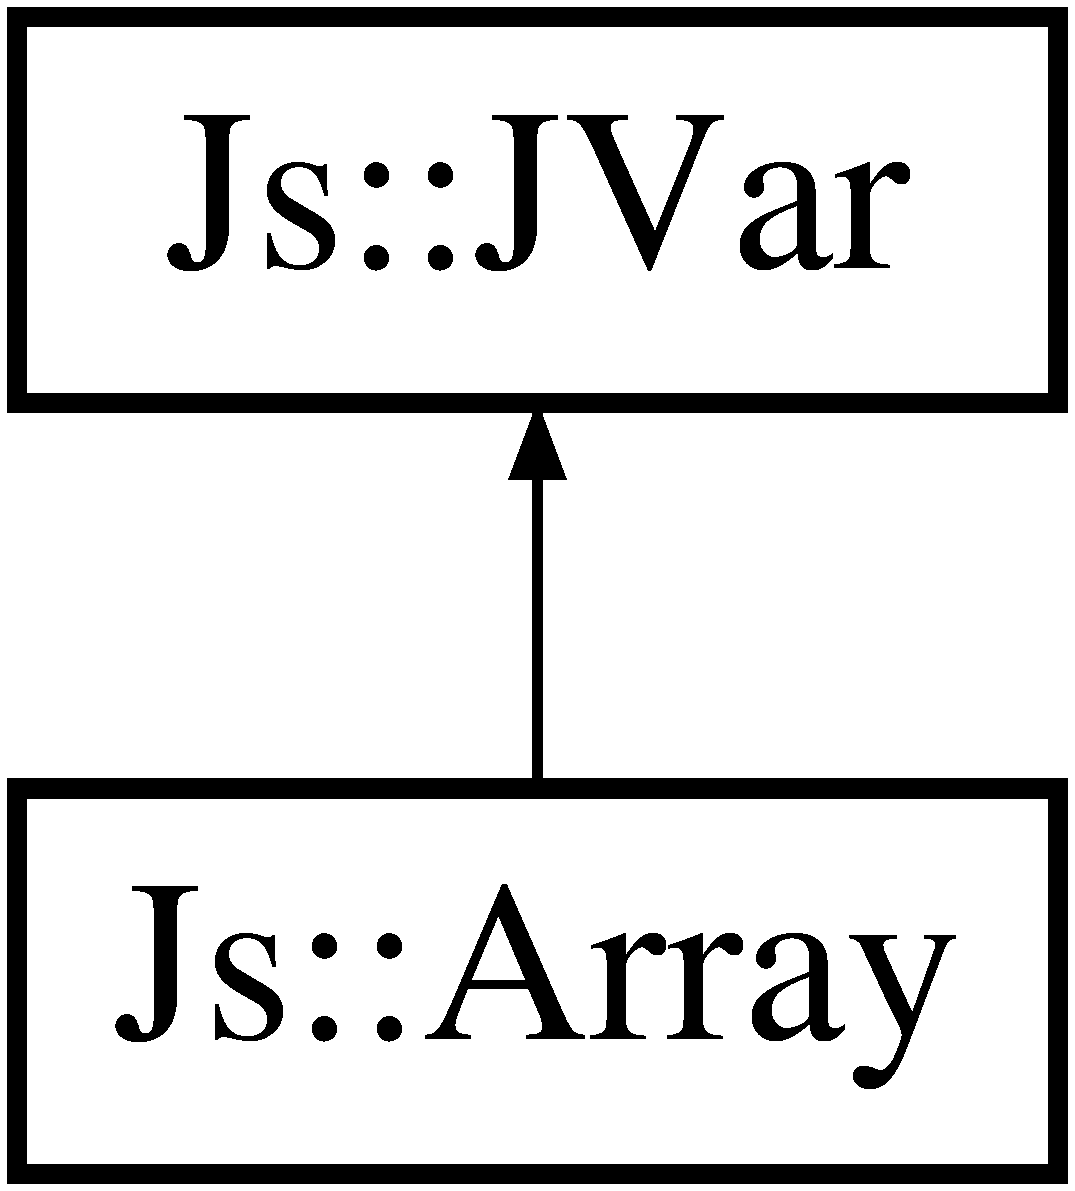
\includegraphics[height=2cm]{classJs_1_1Array}
\end{center}
\end{figure}


\subsection{Detailed Description}
\begin{Desc}
\item[Author:]Neel Basu $<$neel$>$ \end{Desc}


The documentation for this class was generated from the following files:\begin{CompactItemize}
\item 
array.h\item 
array.cpp\end{CompactItemize}
